%% wp2 布局：表示、示例、完备性与半线性（论文 2. Layout 小节）

\wpsh{布局}
\label{sec:layout}

\CuTe 使用形状（shape）$S$ 与步幅（stride）$D$ 来定义一个\emph{布局函数}（layout function），或简称\emph{布局}（layout）。形状 $S$ 定义布局函数的定义域（domain），而步幅 $D$ 定义布局函数的陪域（codomain）。

对前文所述形状的另一种解释是：它是从所有坐标（coordinate）列表的集合到自然坐标的一个映射。该映射是双射，因此每个坐标都被映射到形状内一个唯一且等价的自然坐标。类似地，步幅是从某个形状的自然坐标到某个陪域的映射。
\begin{align*}
S \ &\colon \ Z \leftrightarrow \Z_S, \ \forall Z \in \Z(S) \\
D \ &\colon \ \Z_S \to \D
\end{align*}
其中 $\leftrightarrow$ 是 {\tt idx2crd} \eqref{eqn:idx2crd} 与 {\tt crd2idx} \eqref{eqn:crd2idx} 这两个函数，它们在相容形状的自然坐标之间进行映射；而 $\to$ 映射则是自然坐标与步幅之间的 \texttt{inner\_product} \eqref{eqn:innerprod}。

形状与步幅的复合（composition）定义了布局函数，它是从所有坐标列表的集合到陪域的映射。

\begin{definition}
\emph{布局} $\v{L} = D \circ S$ 是形状 $S$ 与步幅 $D$ 的函数复合，其中 $S \sim D$，它为每个 $Z \in \Z(S)$ 定义了一个映射 $Z \to \D$。
\end{definition}

\wpssh{记号与运算}

我们依据上下文以不同的记号书写布局 $\v{L}$。例如：
\begin{align*}
\begin{array}{ccc} (4, & (3, & 2)) \\ (2, & (8, & 1)) \end{array} = \begin{array}{c} S \\ D \end{array} \quad\quad \text{或} \quad\quad (4, (3, 2)) : (2, (8, 1)) = S : D  \quad\quad \text{或} \quad\quad (2, (8, 1)) \circ (4, (3, 2)) = D \circ S
\end{align*}
其中最后一种写法强调：形状与步幅本身也可以被解释为函数，它们复合起来定义布局函数。

由于布局的定义域由其形状决定，布局的性质与形状的性质紧密对齐。对于布局 $\v{L} = S : D$ 与 $\v{U} = X : Y$，我们定义：
\begin{compactitem}
\item $\text{阶}(\v{L}) = \text{阶}(S)$：布局的阶（rank）是其形状的阶。
\item $\text{深度}(\v{L}) = \text{深度}(S)$：布局的深度（depth）是其形状的深度。
\item $\abs{\v{L}} = \abs{S}$：布局的大小是其形状的大小。
\item $\v{L}_i = S_i : D_i$：第 $i$ 个子布局（sublayout）由其形状与步幅的第 $i$ 个元素构成。
\item $\Z(\v{L}) = \Z(S)$：布局的坐标集合是其形状的坐标集合。
\item $\v{L} \sim \v{U} \Leftrightarrow S \sim X$：两个布局的同构（congruent）关系是其形状的同构关系。
\item $\v{L} \preceq \v{U} \Leftrightarrow S \preceq X$：两个布局的相容性是其形状的相容性。
\end{compactitem}

作为布局求值的一个例子，考虑图~\ref{fig:layouts:mixed} 中的布局 $\v{L} = ((2,2),(4,2)):((1,8),(2,16))$ 以及整数坐标 $22 \in Z_{32} \in Z(\v{L})$，则
\begin{align*}
\v{L}(22) = \v{L}(2,5) = \v{L}((0,1),(1,1)) = 26
\end{align*}
其中我们依次展示了整数坐标、等价的二维坐标、等价的自然坐标以及计算得到的偏移。

布局的界内定义域是所有坐标 $c \in \Z(\v{L})$ 的集合。布局也可以在越界坐标上求值，这类似于可以在越界索引上求值但行为未定义的数组。因此，布局的定义域是有限集合 $\Z(\v{L})$，而\emph{扩展定义域}（extended domain）是与 $S$ 弱同构的所有 $\texttt{HTuple}(\Z)$ 构成的无穷集合 $\Z^\v{L}$。

我们还区分布局的陪域与像集。布局的陪域是 $\D$，它通常是无穷的（例如 $\Z$ 或 $\Z^D$）。布局的像集是有限的，是布局对其定义域内所有坐标所产生的取值范围。
\begin{align*}
\text{像}(\v{L}) = \v{L}(\Z(\v{L})) = \v{L}(\Z_{\abs{\v{L}}}) \subseteq \text{陪域}(\v{L})
\end{align*}

\wpssh{布局示例}

在定义了形状、步幅与布局之后，我们现在给出一些示例，说明 \CuTe 布局是对常见扁平 N 维布局的严格推广。

\begin{figure}[ht]
\centering
\begin{subfigure}[t]{0.3\textwidth}
    \centering
    \begin{tikzpicture}[thick,scale=1.10, every node/.style={scale=1.10}]
        \draw[step=0.5cm,color=black] (-2,-1) grid (2,1);
        \matrix[matrix of nodes,nodes={inner sep=0pt,text width=.5cm,align=center,minimum height=.5cm}]{
            0 & 4 & 8  & 12 & 16 & 20 & 24 & 28 \\
            1 & 5 & 9  & 13 & 17 & 21 & 25 & 29 \\
            2 & 6 & 10 & 14 & 18 & 22 & 26 & 30 \\
            3 & 7 & 11 & 15 & 19 & 23 & 27 & 31 \\};
        \draw[line width=2pt,rounded corners,opacity=0.2]
        (-1.75,+0.75) -- (-1.75,-0.75) --
        (-1.25,+0.75) -- (-1.25,-0.75) --
        (-0.75,+0.75) -- (-0.75,-0.75) --
        (-0.25,+0.75) -- (-0.25,-0.75) --
        (+0.25,+0.75) -- (+0.25,-0.75) --
        (+0.75,+0.75) -- (+0.75,-0.75) --
        (+1.25,+0.75) -- (+1.25,-0.75) --
        (+1.75,+0.75) -- (+1.75,-0.75);
    \end{tikzpicture}
    \subcaption{\tabular[t]{@{}l@{}}列主序 \\ $(4,8):(1,4)$\endtabular}
\end{subfigure}
\begin{subfigure}[t]{0.3\textwidth}
    \centering
    \begin{tikzpicture}[thick,scale=1.10, every node/.style={scale=1.10}]
        \draw[step=0.5cm,color=black] (-2,-1) grid (2,1);
        \matrix[matrix of nodes,nodes={inner sep=0pt,text width=.5cm,align=center,minimum height=.5cm}]{
            0  & 1  & 2  & 3  & 4  & 5  & 6  & 7  \\
            8  & 9  & 10 & 11 & 12 & 13 & 14 & 15 \\
            16 & 17 & 18 & 19 & 20 & 21 & 22 & 23 \\
            24 & 25 & 26 & 27 & 28 & 29 & 30 & 31 \\};
        \draw[line width=2pt,rounded corners,opacity=0.2]
        (-1.75,+0.75) -- (+1.75,+0.75) --
        (-1.75,+0.25) -- (+1.75,+0.25) --
        (-1.75,-0.25) -- (+1.75,-0.25) --
        (-1.75,-0.75) -- (+1.75,-0.75);
    \end{tikzpicture}
    \subcaption{\tabular[t]{@{}l@{}}行主序 \\ $(4,8):(8,1)$\endtabular}
\end{subfigure}
\begin{subfigure}[t]{0.3\textwidth}
    \centering
    \begin{tikzpicture}[thick,scale=1.10, every node/.style={scale=1.10}]
        \draw[step=0.5cm,color=black] (-2,-1) grid (2,1);
        \matrix[matrix of nodes,nodes={inner sep=0pt,text width=.5cm,align=center,minimum height=.5cm}]{
            0 & 5 & 10 & 15 & 20 & 25 & 30 & 35 \\
            1 & 6 & 11 & 16 & 21 & 26 & 31 & 36 \\
            2 & 7 & 12 & 17 & 22 & 27 & 32 & 37 \\
            3 & 8 & 13 & 18 & 23 & 28 & 33 & 38 \\};
        \draw[line width=2pt,rounded corners,opacity=0.2]
        (-1.75,+0.75) -- (-1.75,-0.75) --
        (-1.25,+0.75) -- (-1.25,-0.75) --
        (-0.75,+0.75) -- (-0.75,-0.75) --
        (-0.25,+0.75) -- (-0.25,-0.75) --
        (+0.25,+0.75) -- (+0.25,-0.75) --
        (+0.75,+0.75) -- (+0.75,-0.75) --
        (+1.25,+0.75) -- (+1.25,-0.75) --
        (+1.75,+0.75) -- (+1.75,-0.75);
    \end{tikzpicture}
    \subcaption{\tabular[t]{@{}l@{}}列主序填充 \\ $(4,8):(1,5)$\endtabular}
\end{subfigure}
\begin{subfigure}[t]{0.3\textwidth}
    \centering
    \begin{tikzpicture}[thick,scale=1.10, every node/.style={scale=1.10}]
        \draw[step=0.5cm,color=black] (-2,-1) grid (2,1);
        \matrix[matrix of nodes,nodes={inner sep=0pt,text width=.5cm,align=center,minimum height=.5cm}]{
            0  & 1  & 2  & 3  & 16 & 17 & 18 & 19 \\
            4  & 5  & 6  & 7  & 20 & 21 & 22 & 23 \\
            8  & 9  & 10 & 11 & 24 & 25 & 26 & 27 \\
            12 & 13 & 14 & 15 & 28 & 29 & 30 & 31 \\};
        \draw[line width=2pt,rounded corners,opacity=0.2]
        (-1.75,+0.75) -- (-0.25,+0.75) --
        (-1.75,+0.25) -- (-0.25,+0.25) --
        (-1.75,-0.25) -- (-0.25,-0.25) --
        (-1.75,-0.75) -- (-0.25,-0.75) --
        (+0.25,+0.75) -- (+1.75,+0.75) --
        (+0.25,+0.25) -- (+1.75,+0.25) --
        (+0.25,-0.25) -- (+1.75,-0.25) --
        (+0.25,-0.75) -- (+1.75,-0.75);
    \end{tikzpicture}
    \subcaption{\tabular[t]{@{}l@{}}列主序交错 \\ $(4,(4,2)):(4,(1,16))$\endtabular}
\end{subfigure}
\begin{subfigure}[t]{0.3\textwidth}
    \centering
    \begin{tikzpicture}[thick,scale=1.10, every node/.style={scale=1.10}]
        \draw[step=0.5cm,color=black] (-2,-1) grid (2,1);
        \matrix[matrix of nodes,nodes={inner sep=0pt,text width=.5cm,align=center,minimum height=.5cm}]{
            0  & 2  & 4  & 6  & 16 & 18 & 20 & 21 \\
            1  & 3  & 5  & 7  & 17 & 19 & 22 & 23 \\
            8  & 10 & 12 & 14 & 24 & 26 & 28 & 30 \\
            9  & 11 & 13 & 15 & 25 & 27 & 29 & 31 \\};
        \draw[line width=2pt,rounded corners,opacity=0.2]
        (-1.75,+0.75) -- (-1.75,+0.25) --
        (-1.25,+0.75) -- (-1.25,+0.25) --
        (-0.75,+0.75) -- (-0.75,+0.25) --
        (-0.25,+0.75) -- (-0.25,+0.25) --
        (-1.75,-0.25) -- (-1.75,-0.75) --
        (-1.25,-0.25) -- (-1.25,-0.75) --
        (-0.75,-0.25) -- (-0.75,-0.75) --
        (-0.25,-0.25) -- (-0.25,-0.75) --
        (+0.25,+0.75) -- (+0.25,+0.25) --
        (+0.75,+0.75) -- (+0.75,+0.25) --
        (+1.25,+0.75) -- (+1.25,+0.25) --
        (+1.75,+0.75) -- (+1.75,+0.25) --
        (+0.25,-0.25) -- (+0.25,-0.75) --
        (+0.75,-0.25) -- (+0.75,-0.75) --
        (+1.25,-0.25) -- (+1.25,-0.75) --
        (+1.75,-0.25) -- (+1.75,-0.75);
    \end{tikzpicture}
    \subcaption{\tabular[t]{@{}l@{}}混合 \\ $((2,2),(4,2)):((1,8),(2,16))$\endtabular}
  \label{fig:layouts:mixed}
\end{subfigure}
\begin{subfigure}[t]{0.3\textwidth}
    \centering
    \begin{tikzpicture}[thick,scale=1.10, every node/.style={scale=1.10}]
        \draw[step=0.5cm,color=black] (-2,-1) grid (2,1);
        \matrix[matrix of nodes,nodes={inner sep=0pt,text width=.5cm,align=center,minimum height=.5cm}]{
            0  & 0  & 4  & 4  & 8  & 8  & 12  & 12  \\
            0  & 0  & 4  & 4  & 8  & 8  & 12  & 12  \\
            2  & 2  & 6  & 6  & 10 & 10 & 14  & 14  \\
            2  & 2  & 6  & 6  & 10 & 10 & 14  & 14  \\};
        \draw[line width=2pt,rounded corners,opacity=0.2]
        (-1.75,+0.75) --
        (-1.75,-0.25) --
        (-0.75,+0.75) --
        (-0.75,-0.25) --
        (+0.25,+0.75) --
        (+0.25,-0.25) --
        (+1.25,+0.75) --
        (+1.25,-0.25);
    \end{tikzpicture}
    \subcaption{\tabular[t]{@{}l@{}}块状广播 \\ $((2,2),(2,4)):((0,2),(0,4))$\endtabular}
  \label{fig:layouts:broadcast}
\end{subfigure}
\caption{与形状 $(4,8)$ 相容的布局示例，绘制为 $4 {\times} 8$ 矩阵。这些布局使用整数步幅与层次形状（hierarchical shapes）来定义对数据张量有用的函数。浅色线条沿布局偏移的总体顺序勾勒。}
\label{fig:layouts}
\end{figure}

图~\ref{fig:layouts} 展示了稠密线性代数库（如 CUTLASS）中常见的数据布局示例。每个布局都被表示为从逻辑坐标 $(m,n) \in \Z_{(4,8)}$ 到偏移 $k \in \Z$ 的映射。例如，这些偏移可用于索引数据数组中的元素。常见的行主序（row-major）、列主序（column-major）与填充（padded）布局都可以平凡地用 \CuTe 布局表示，而交错（interleaved）与混合（mixed）布局则表明：通过使用嵌套的形状与步幅，布局的表示集合被严格地扩大。特别地，可以清楚地看到，由数据块构成的网格（grids-of-tiles-of-data）可以直接用 \CuTe 布局表示。

\begin{figure}[ht]
\centering
\begin{subfigure}[t]{0.45\textwidth}
    \centering
    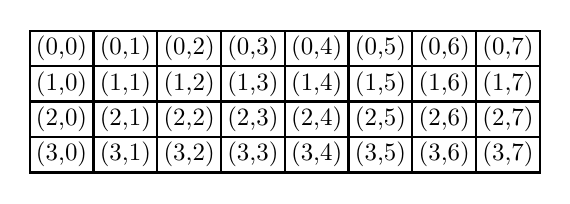
\begin{tikzpicture}[thick,scale=0.9, every node/.style={scale=0.9}]
      \foreach \row in {0,...,3} {
        \foreach \col in {0,...,7} {
          \draw (0.9*\col,-0.5*\row) rectangle ++(0.9,-0.5) node[pos=.5] {(\row,\col)};
        }
      }
    \end{tikzpicture}
    \subcaption{\tabular[t]{@{}l@{}}恒等坐标 \\ $(4,8):(e_0,e_1)$\endtabular}
    \label{fig:layouts:coord0}
\end{subfigure}
\begin{subfigure}[t]{0.45\textwidth}
    \centering
    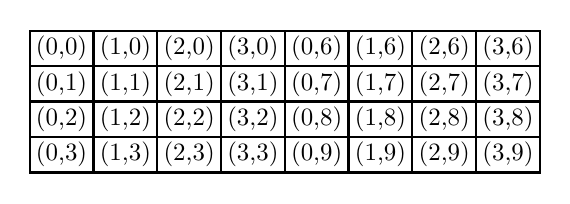
\begin{tikzpicture}[thick,scale=0.9, every node/.style={scale=0.9}]
      \foreach \row in {0,...,3} {
        \foreach \cola in {0,...,3} {
          \foreach \colb in {0,...,1} {
            \pgfmathtruncatemacro{\secondcoord}{\row + 6*\colb}
            \draw (0.9*\cola+3.6*\colb,-0.5*\row) rectangle ++(0.9,-0.5) node[pos=.5] {(\cola,\secondcoord)};
          }
        }
      }
    \end{tikzpicture}
    \subcaption{\tabular[t]{@{}l@{}}转置块状坐标 \\ $(4,(4,2)):(e_1,(e_0,6e_1))$\endtabular}
    \label{fig:layouts:coord1}
\end{subfigure}
%\begin{subfigure}[t]{0.7\textwidth}
%    \centering
%    \begin{tikzpicture}[thick,scale=0.9, every node/.style={scale=0.9}]
%      \foreach \row in {0,...,3} {
%        \foreach \col in {0,...,7} {
%          \pgfmathparse{int(mod(\row,2))}\let\i\pgfmathresult
%          \pgfmathparse{int(mod(\col,2))}\let\j\pgfmathresult
%          \pgfmathparse{int(int(\col/2) + 4*int(\row/2))}\let\k\pgfmathresult
%          \draw (1.3*\col,-0.5*\row) rectangle ++(1.3,-0.5) node[pos=.5] {(\i,\j,\k)};
%        }
%      }
%    \end{tikzpicture}
%    \caption{折叠坐标布局 \\ $((2,2),(2,4)):((e_0,4e_2),(e_1,e_2))$}
%\end{subfigure}
\begin{subfigure}[t]{0.45\textwidth}
    \centering
    \begin{tikzpicture}[thick,scale=1, every node/.style={scale=1}]
        \draw[step=0.5cm,color=black] (-3,-1) grid (3,1);
        \matrix[matrix of nodes,nodes={inner sep=0pt,text width=.5cm,align=center,minimum height=.5cm}]{
            0 & 5 & 10 & 15 & 16 & 21 & 26 & 31 & 32 & 37 & 42 & 47 \\
            1 & 4 & 11 & 14 & 17 & 20 & 27 & 30 & 33 & 36 & 43 & 46 \\
            2 & 7 &  8 & 13 & 18 & 23 & 24 & 29 & 34 & 39 & 40 & 45 \\
            3 & 6 &  9 & 12 & 19 & 22 & 25 & 28 & 35 & 38 & 41 & 44 \\};
        % \draw[line width=2pt,rounded corners,opacity=0.2]
        % (-1.75,+0.75) -- (-1.75,-0.75) --
        % (-1.25,+0.75) -- (-1.25,-0.75) --
        % (-0.75,+0.75) -- (-0.75,-0.75) --
        % (-0.25,+0.75) -- (-0.25,-0.75) --
        % (+0.25,+0.75) -- (+0.25,-0.75) --
        % (+0.75,+0.75) -- (+0.75,-0.75) --
        % (+1.25,+0.75) -- (+1.25,-0.75) --
        % (+1.75,+0.75) -- (+1.75,-0.75);
    \end{tikzpicture}
    \subcaption{\tabular[t]{@{}l@{}}二进制 Swizzle \\ $(4,(4,3)):(f_1,(f_5,f_{16}))$ \\ $f_i \in F_2 = (\Z,XOR,\cdot)$\endtabular}
    \label{fig:layouts:swizzle}
\end{subfigure}
\caption{以二维坐标绘制的布局示例。这些布局使用来自整数半模（integer-semimodule）的步幅来定义函数，这些函数在跟踪坐标以及按非仿射（non-affine）模式对偏移做“混淆（swizzle）”处理时非常有用。}
\label{fig:layouts2}
\end{figure}

图~\ref{fig:layouts2} 展示了用整数半模步幅而非整数步幅构造的布局示例。图~\ref{fig:layouts:coord0} 与图~\ref{fig:layouts:coord1} 演示了生成坐标的布局。在后续章节中我们将发现，这些坐标布局与其对应的数据布局对称地变换，并且常常作为检测数据张量越界访问并对其进行谓词化（predicating）的实用工具。此外，坐标张量已被证明对于 Hopper 与 Blackwell 中诸如 TMA 这类以坐标而非地址作为指令参数的指令非常有用。图~\ref{fig:layouts:swizzle} 使用了一个以二进制 XOR 替换群加法的整数半模。它可用于生成所谓的 swizzle 模式，这类模式有助于避免对共享内存读写访问模式中的 bank 冲突。这些示例突显了 \CuTe 布局概念的统一性以及它所能表示函数的普适性。

\wpssh{完备性}

任何满足 $f(0) = 0$ 且定义域为有限集合 $\Z_N$ 的函数 $f$ 都可以表示为有限个 \CuTe 布局的函数复合。这意味着 \CuTe 布局在函数复合下构成一个生成集。这样的函数 $f$ 可以表示为如下复合序列
\begin{align*}
f &\equiv (2,2,2,\ldots):(f(1),f(2),f(3),\ldots) \ \circ \ (3,1):(1,4) \ \circ \ (4,1):(1,6) \ \circ \ \cdots \ \circ \ (N-1,1):(1,2(N-2)).
\end{align*}
对所有 $i \in \Z_N / \{0\}$，最右边的 $N-3$ 个布局将 $i \to 2^{i-1}$，而最左边的布局将 $2^{i-1} \to f(i)$。注意，我们在上面求值中间布局时使用的是扩展定义域 $\Z$，而不是界内定义域 $\Z_N$。

\wpssh{半线性}

形状—步幅定义 $\v{L} = D \circ S$ 连同推广的整数模（integer-module）步幅，给出了布局函数一种特别有用的线性代数视角，
\begin{align}
\v{L}(c) = (D \circ S)(c) = d \cdot S(c) = d \cdot \tilde{c}.
\end{align}
形状函数是到自然坐标 $\tilde{c} \in \Z^S$ 的一个便利的半仿射双射，而步幅函数是自然坐标的线性函数。事实上，对于两个自然坐标 $\tilde{c}_0, \tilde{c}_1 \in \Z^S$，布局函数是线性（linear）的，
\begin{align*}
\v{L}(\alpha \tilde{c}_0 + \beta \tilde{c}_1) = d \cdot (\alpha \tilde{c}_0 + \beta \tilde{c}_1) = \alpha (d \cdot \tilde{c}_0) + \beta (d \cdot \tilde{c}_1) = \alpha \v{L}(\tilde{c}_0) + \beta \v{L}(\tilde{c}_1),
\end{align*}
因为形状函数是恒等映射且步幅函数是线性的。注意，对任意坐标 $c_0, c_1 \in \Z(S)$，布局不是线性的，因为形状函数不是线性的，
\begin{align*}
\tilde{c} = S(c_0 + c_1) \neq S(c_0) + S(c_1) = \tilde{c}_0 + \tilde{c}_1.
\end{align*}
因此，布局函数在自然坐标 $\tilde{c} \in \Z^S$ 下是线性的，但在任意坐标 $c \in \Z(S)$ 下是非线性的。

在自然坐标下，$d \cdot \tilde{c}$ 可以解释为推广的矩阵—向量乘积（matrix-vector product），
\begin{align*}
\v{L}(c) = d \cdot \tilde{c} = \v{D} \ \tilde{c}
\end{align*}
其中 $\v{D}$ 是元素取自某个整数半模 $\D$ 的矩阵。在最常见的整数步幅情形下，$\D = \Z$，这是 $\v{D} \in \Z^{1 \times n}$ 的矩阵—向量乘积。当步幅取自坐标整数半模 $\D = (\Z^S, +, \cdot)$ 时，这是 $\v{D} \in \Z^{m \times n}$ 的矩阵—向量乘积。当步幅是二进制序列时，$\D = F_2^m = (\Z_{2^m}, XOR, \cdot)$，这是 $\v{D} \in \mathbb{F}_2^{m \times n}$ 的矩阵—向量乘积。

\begin{table}[ht]
\begin{center}
\begin{tabular}{|>{$}c<{$}|>{$}c<{$}|c|}
\v{L} & \text{线性形式：} r = \v{D} \ \tilde{c} & 说明 \\ \hline \hline
((2,2),(4,\ 2)):((1,8),(2,16)) & r = \begin{bmatrix}1 & 8 & 2 & 16\end{bmatrix} \begin{bmatrix} \tilde{c}_0 \\ \tilde{c}_1 \\ \tilde{c}_2 \\ \tilde{c}_3 \end{bmatrix} & \shortstack{整数步幅是\\ $1 {\times} n$ $\Z$-矩阵的列} \\ \hline
(4,(4,2)):(e_1,(e_0,6e_1)) & \begin{bmatrix}r_0 \\ r_1\end{bmatrix} = \begin{bmatrix}0 & 1 & 0 \\ 1 & 0 & 6 \end{bmatrix} \begin{bmatrix} \tilde{c}_0 \\ \tilde{c}_1 \\ \tilde{c}_2 \end{bmatrix} &
\shortstack{坐标步幅是\\ $m {\times} n$ $\Z$-矩阵的列} \\ \hline
\shortstack{$(4,4) : (f_1,f_5)$ \\ $\equiv ((2,2),(2,2)):((f_1,f_2),(f_5,f_{10}))$} &
\footnotesize
\begin{bmatrix}r_0 \\ r_1 \\ r_2 \\ r_3\end{bmatrix} =
\begin{bmatrix}
1 & 0 & 1 & 0 \\
0 & 1 & 0 & 1 \\
0 & 0 & 1 & 0 \\
0 & 0 & 0 & 1 \\
\end{bmatrix}
\begin{bmatrix} \tilde{c}_0 \\ \tilde{c}_1 \\ \tilde{c}_2 \\ \tilde{c}_3 \end{bmatrix} &
\shortstack{二进制步幅是\\ $m {\times} n$ $\mathbb{F}_2$-矩阵的列} \\ \hline
\end{tabular}
\end{center}
\caption{布局及其对应的线性形式。}
\label{tab:linear_forms}
\end{table}

例如，表~\ref{tab:linear_forms} 展示了一个整数布局、一个坐标布局与一个二进制布局的线性形式。针对 $\mathbb{F}_2$ 线性形式已被充分研究的变换包括位排列补（Bit Permute Complement，BPC）与位矩阵乘补（Bit Matrix Multiply Complement，BMMC）变换（Edelman 等，1994；Cormen，1993；Bouverot-Dupuis 与 Sheeran，2023），它们近来在 SIMT GPU 编程中获得了重要的应用（Zhou 等，2025）。在这些工作中，所考虑的变换为
\begin{align}
f(\v{v}) = \v{A} \v{v} + \v{b}
\label{eqn:linear}
\end{align}
其中 $\v{A}$ 是一个 $m {\times} n$ 的二进制元素矩阵，$\v{v}$ 是长度为 $n$ 的二进制向量，$\v{b}$ 是长度为 $m$ 的二进制向量，且所有算术都以 2 为模（在只有两个元素的有限域 $\mathbb{F}_2$ 中）执行。

本文的后续章节将定义 \CuTe 布局上的代数运算，这些运算是从线性代数推广而来的。\CuTe 布局上的群复合可以解释为矩阵乘法的推广。\CuTe 布局的右逆与左逆可以解释为线性代数中的 Moore-Penrose 伪逆。事实上，在 BCP 与 BMMC 分析中也可以找到类似的线性代数表达式（Edelman 等，1994；Cormen，1993；Bouverot-Dupuis 与 Sheeran，2023；Zhou 等，2025），它们都在算法分析中使用分解、逆与矩阵乘积。\CuTe 布局代数可以解释为线性代数的 BCP 与 BMMC 运算向 $\mathbb{F}_2$ 域之外的推广。特别地，\CuTe 布局代数的主要动机来自张量异构数据布局中常见的一般整数步幅。在本工作中，我们旨在证明：这些运算更一般的函数式定义对 \CuTe 布局而言通常是可计算的，并且对广泛的分析与应用都是有用的。
